\documentclass[main.tex]{subfiles}

\begin{document}

\section{A4 Smartphone}
Modellieren Sie die folgende Steuerung für ein Smartphone als UML-Zustandsdiagramm:

\begin{enumerate}
    \item Das Smartphone kann sich in den Zuständen Ausgeschaltet, Standby, Energiesparen und Normal befinden.
    \item Ereignisse für Zustandsübergänge sind das Drücken der An/Aus-Taste, der Home-Taste oder eine Bildschirmgeste. Diese Ereignisse sollen als Signale modelliert werden.
    \item Nach 15 Sekunden Inaktivität im Normalzustand wird der Energiesparmodus aktiviert. Dieser kann durch Drücken der Home-Taste beendet werden.
    \item Nach 60 Sekunden im Energiesparmodus wird der Standby-Betrieb aktiviert. Durch Drücken der Home-Taste gelangt man wieder in den Normalbetrieb.
    \item Das Smartphone kann im Normalbetrieb über die An/Aus-Taste ausgeschaltet werden. Ist das Smartphone ausgeschaltet, dann kann es über die An/Aus-Taste eingeschaltet werden und man gelangt in den Normalbetrieb.
\end{enumerate}

\subsection{Lösung 4}

\begin{figure}[h!]
    \makebox[\textwidth][c]{
        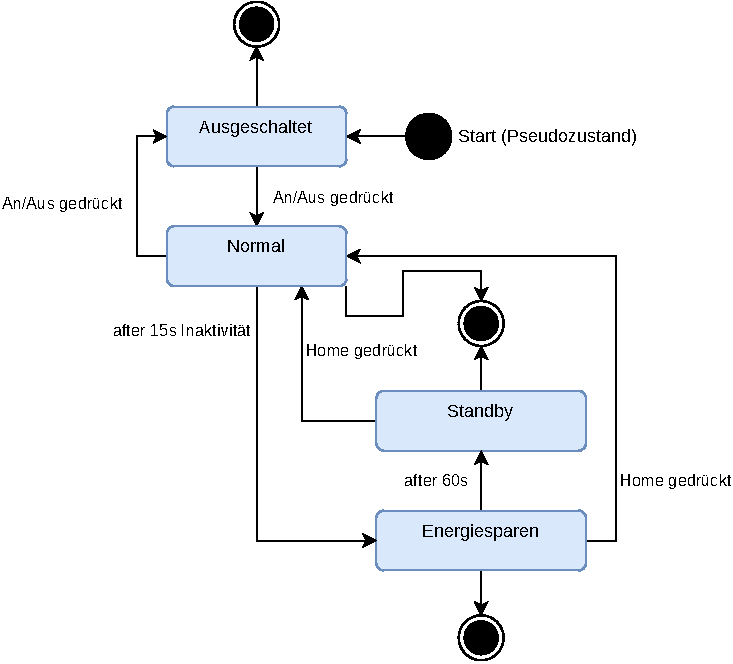
\includegraphics[width=1\linewidth]{h04_A4.drawio.pdf}
    }
    \caption{Smartphone Steuerung}
    \label{fig:lgs4}
\end{figure}

\end{document}
